%%%%%%%%%%%%%%%%%%%%%%%%%%%%%%%%%%%%%%%%%%%%%%%%%%%%%%%%%%%%%%%%%%%%%%
% Problem statement
\begin{statement}[
  problempoints=110,
  timelimit=2 seconds,
  memorylimit=512 MiB,
]{Trener}

\setlength\intextsep{-0.1cm}
\begin{wrapfigure}[7]{r}{0.27\textwidth}
\centering
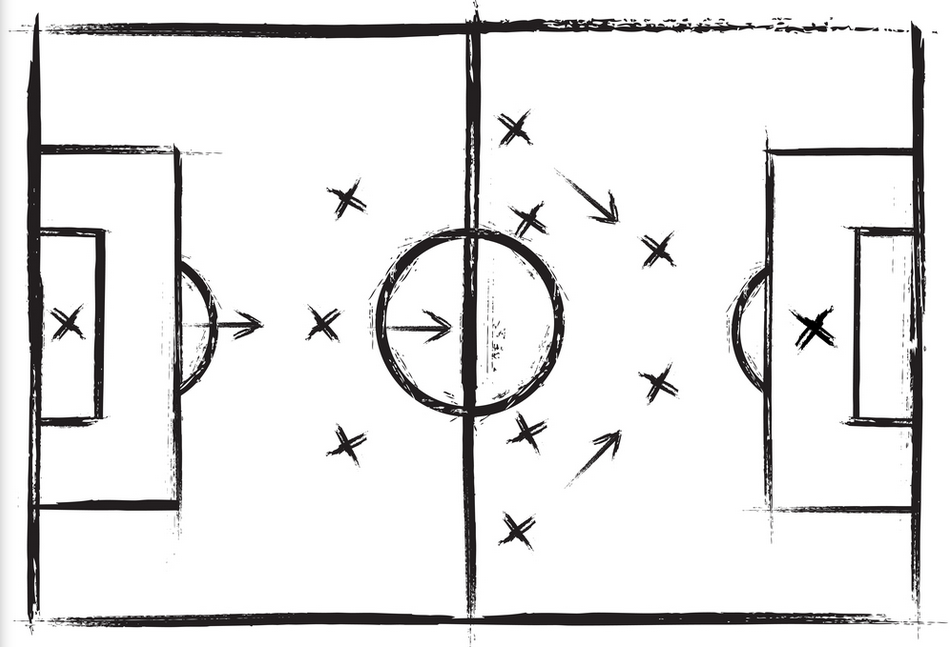
\includegraphics[width=0.27\textwidth]{img/trener.png}
\end{wrapfigure}

At this point we already know that students love to sleep. Patrik is a record
holder in this category. He wakes up only when he needs to eat or if he
wishes to play \textit{FIFA 20}. Therefore, his dreams usually revolve around
football. In his last dream, he found himself in the role of a football manager
of his favourite team -- GNK Dinamo Zagreb.

His job is to select $N$ players that will defend the blue colors in the next
season, but the board has some peculiar requests. They are:

\begin{itemize}
  \item All players must have surnames of distinct lengths.
  \item Surname of a player must appear as a continuous subsequence of surnames
        of all players whose surnames are longer.
\end{itemize}

To make his job easier, Patrik divided the potential players in $N$ buckets
such that players in $i$-th bucket have exactly $i$ letters in their surname.
In each of these buckets there are exactly $K$ players. Patrik wants to know
in how many distinct ways (modulo $10^9 + 7$) can he choose the players for
his squad while also conforming to the given requests.

%%%%%%%%%%%%%%%%%%%%%%%%%%%%%%%%%%%%%%%%%%%%%%%%%%%%%%%%%%%%%%%%%%%%%%
% Input
\subsection*{Input}
The first line contains two integers $N$ $(1 \le N \le 50)$ and $K$ $(1 \le K \le 1\
500)$.

Each of the next $N$ lines contains $K$ not necessarily distinct surnames of
players. The surnames of players in $i$-th of those lines consist of exactly
$i$ lowercase letters from the English alphabet.

%%%%%%%%%%%%%%%%%%%%%%%%%%%%%%%%%%%%%%%%%%%%%%%%%%%%%%%%%%%%%%%%%%%%%%
% Output
\subsection*{Output}
In the only line you should output the answer from the task description.

%%%%%%%%%%%%%%%%%%%%%%%%%%%%%%%%%%%%%%%%%%%%%%%%%%%%%%%%%%%%%%%%%%%%%%
% Scoring
\subsection*{Bodovanje}
{\renewcommand{\arraystretch}{1.4}
  \setlength{\tabcolsep}{6pt}
  \begin{tabular}{ccl}
 Subtask & Score & Constraints \\ \midrule
  1 & 22 & $N = 5$ and $K = 10$ \\
  2 & 33 & $N = 50$ and $K = 100$\\
  3 & 55 & No additional constraints. \\
\end{tabular}}

%%%%%%%%%%%%%%%%%%%%%%%%%%%%%%%%%%%%%%%%%%%%%%%%%%%%%%%%%%%%%%%%%%%%%%
% Examples
\subsection*{Examples}
\begin{tabularx}{\textwidth}{X'X'X}
\sampleinputs{test/trener.dummy.in.1}{test/trener.dummy.out.1} &
\sampleinputs{test/trener.dummy.in.2}{test/trener.dummy.out.2} &
\sampleinputs{test/trener.dummy.in.3}{test/trener.dummy.out.3}
\end{tabularx}

\textbf{Clarification of the first example:}
Patrik can choose the following teams:
\texttt{(a, ab, abc)}, \texttt{(a, ab, abd)},
\texttt{(b, ab, abc)}, \texttt{(b, ab, abd)} and \texttt{(b, bd, abd)}.

%%%%%%%%%%%%%%%%%%%%%%%%%%%%%%%%%%%%%%%%%%%%%%%%%%%%%%%%%%%%%%%%%%%%%%
% We're done
\end{statement}

%%% Local Variables:
%%% mode: latex
%%% mode: flyspell
%%% ispell-local-dictionary: "croatian"
%%% TeX-master: "../hio.tex"
%%% End:
